\documentclass[12pt]{article}   % artigo fonte 12
\usepackage[
a4paper,		% papel A4
left=1.5cm,		% margem esquerda
right=1.5cm,		% margem direita
top=1.5cm,		% margem superior
bottom=1.5cm		% margem inferior
]{geometry}
% Caracteres / Acentos / Português do Brasil
\usepackage[utf8]{inputenc}
\usepackage[T1]{fontenc}	
\usepackage[brazil]{babel}
% Pacotes Matemática
\usepackage{array,latexsym}
\usepackage{amsmath,amsfonts,amssymb,amsthm,mathabx,amstext}
\usepackage{dsfont}	% Conjuntos: $\mathds{N, Z, Q, R, C}$
\usepackage{graphicx}

\begin{document}
	
	\begin{figure}[h!]
		
\includegraphics[scale=0.7]{ufpbde}
		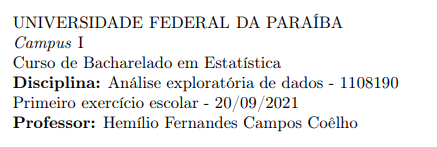
\includegraphics[scale=0.7]{ufpbhemilio}
	\end{figure}

\par \textbf{Aluno:} \underline{Paulo Ricardo Seganfredo Campana}
\vspace{+12pt}
\par \textbf{Questão 1}
\vspace{+12pt}
\par 01.(V) verdadeira, pois a moda representa o ponto mais alto do histograma, se a moda é maior que a mediana e a média, temos um coeficiente de assimetria negativo, que compreende valores aglutinados a direita.
\par 02.(V) verdadeira, pois uma população pode ser um conjunto de diversos outros objetos ou eventos com características de interesse, a população por exemplo, pode ser um conjunto de automóveis, ou um conjunto de incêndios.
\par 03.(V) verdadeira, pois é natural que o dado sofra variação aleatória.
\par 04.(V) verdadeira, pois $\overline{X}>M_{d}$, confira: 
\vspace{+6pt}
\par $\overline{X} = \dfrac{1+4+8+0}{4} = 3.25$,
\vspace{+6pt}
\par $\overline{X_G} = \sqrt{1*4*8*0} = 0$
\vspace{+6pt}
\par 05.(V) verdadeiro, pois é definida como o valor que ocorre com maior frequência.
\par 06.(F) falsa, pois a fonte de um dado é indispensável para a veracidade do mesmo.
\par 07.(V) verdadeira, as variáveis quantitativas discretas assumem valores dos números naturais, as quantitativas contínuas podem assumir valores fracionários, já as qualitativas, atribuem informação a variável, com as ordenais podendo ser postas em ordem e as nominais não.
\par 08.(V) verdadeira, pois uma amostra pode conter todos os valores iguais a $0$ ou se permitir valores negativos, uma soma igual a 0.
\par 09.(F) falso, observe o exemplo:
\vspace{+6pt}
\par $(3,5,5,5,7)$
\par $\overline{X} = 5$
\par $M_o = 5$
\par $M_d = 5 \neq 0$
\par a média e a moda assumem mesmos valores, porém a mediana é diferente de zero.
\par 10.(F) falso, pois é possível calcular pela moda de Pearson $M_o = 3M_d - 2\overline{X}$, com $\overline{X} = 0$ e $M_d > 0$ a moda será positiva.
\vspace{+12pt}
\par \textbf{Questão 2}
\vspace{+12pt}
\par (a) O resultado é esperado, $\overline{X} \geq \overline{X_G}$ pela desigualdade das médias, e a média harmônica menor que as duas devido ao menor efeito de valores outliers como 3.9 e 3.7.
\vspace{+6pt}
\par $\dfrac{3.9+2.2+3.7+2.5+2.4+2.3+2.5+2+2+1.4}{10} = 2.49$
\vspace{+6pt}
\par $(3.9*2.2*3.7*2.5*2.4*2.3*2.5*2*2*1.4)^{0.1} = 2.39$
\vspace{+6pt}
\par $\dfrac{n}{\sum_{1}^{10} \dfrac{1}{X_i}} = 2.3$
\vspace{+6pt}
\par (b) $M_d = 2.35, M_o = 2.07$, a mediana é estritamente realista, pois foram usados dados diretamente do rol, já a moda de Pearson assume valor fracionário, porém realistas, já que o rol contem dois elementos de valor $2.0$.
\vspace{+6pt}
\par $M_d = \dfrac{X_{(5)} + X_{(6)}}{2} = \dfrac{2.3 + 2.4}{2} = 2.35$
\vspace{+6pt}
\par $M_o = 3M_d - 2\overline{X} = 3*2.35 - 2*2.49 = 2.07$
\vspace{+6pt}
\par (c)
	\begin{figure}[h!]
		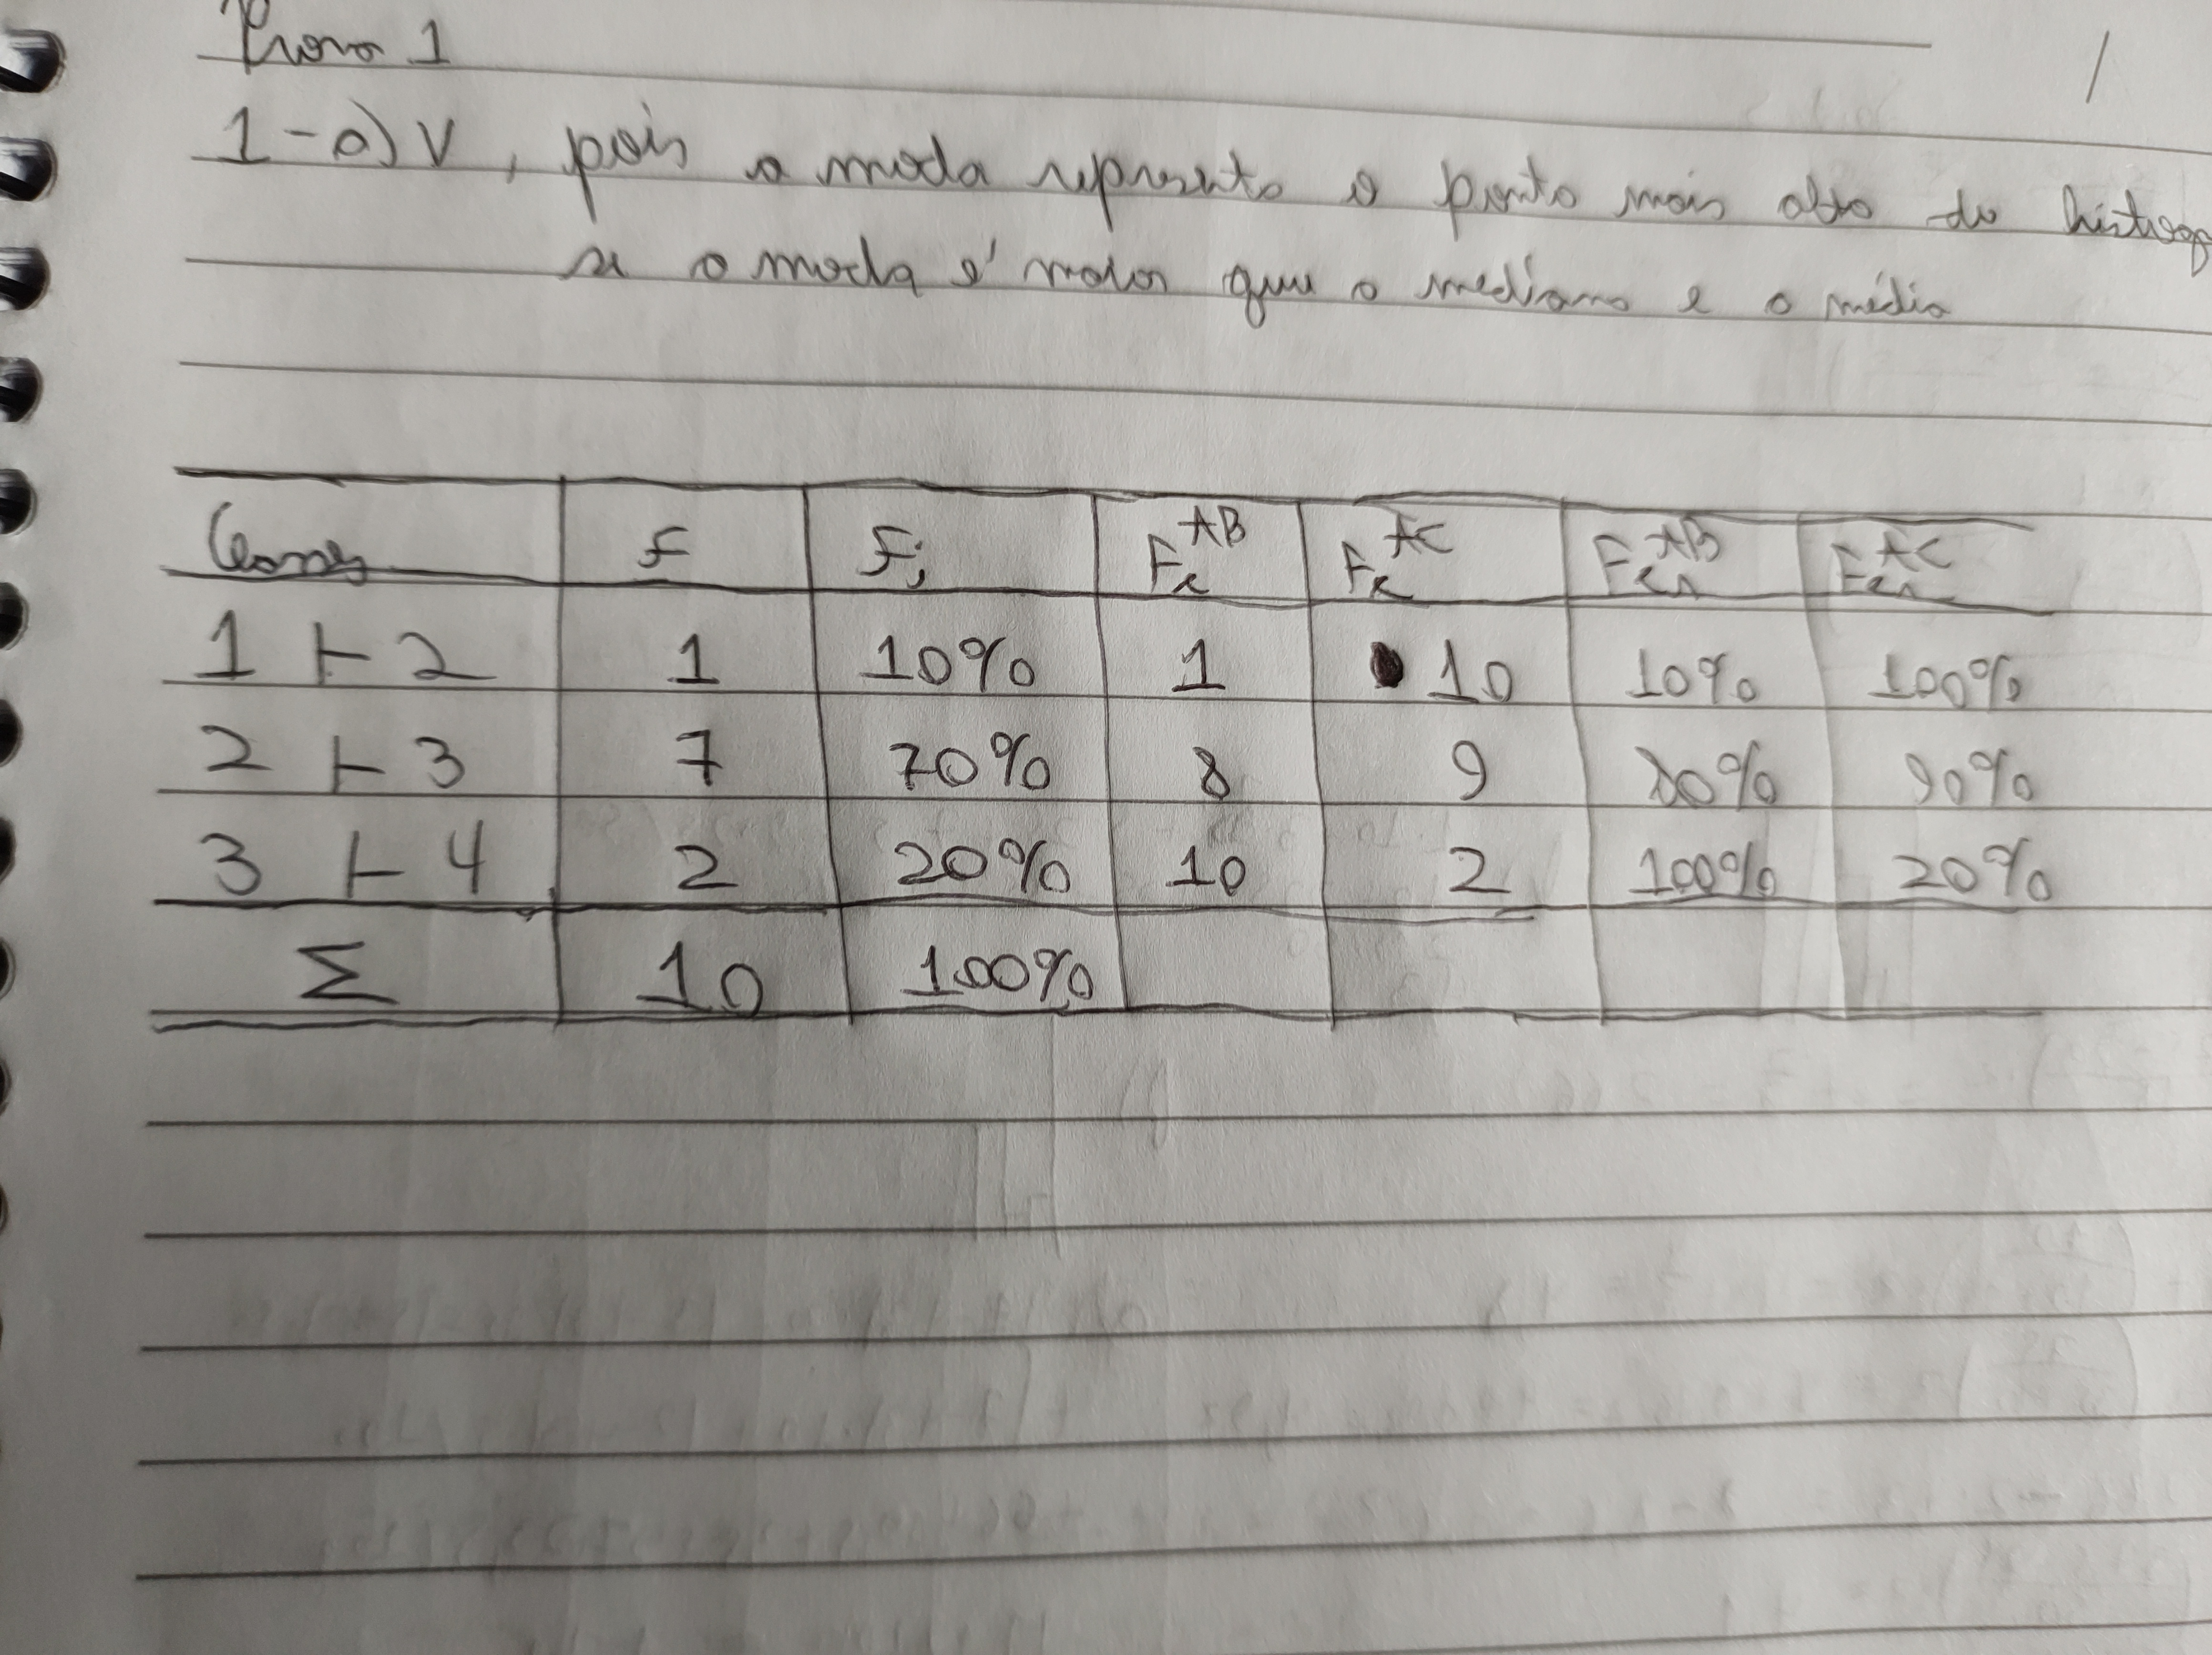
\includegraphics[scale=0.05]{q2c}
	\end{figure}
\par (d) observa-se a grande quantidade de dados no intervalo $2 \vdash 3$, talvez a escolha de classes não foi a melhor, pois não representa o vazio entre os valores $2.6$ a $3.0$, e a distribuição entre $2.0$ e $2.5$.
	\begin{figure}[h!]
		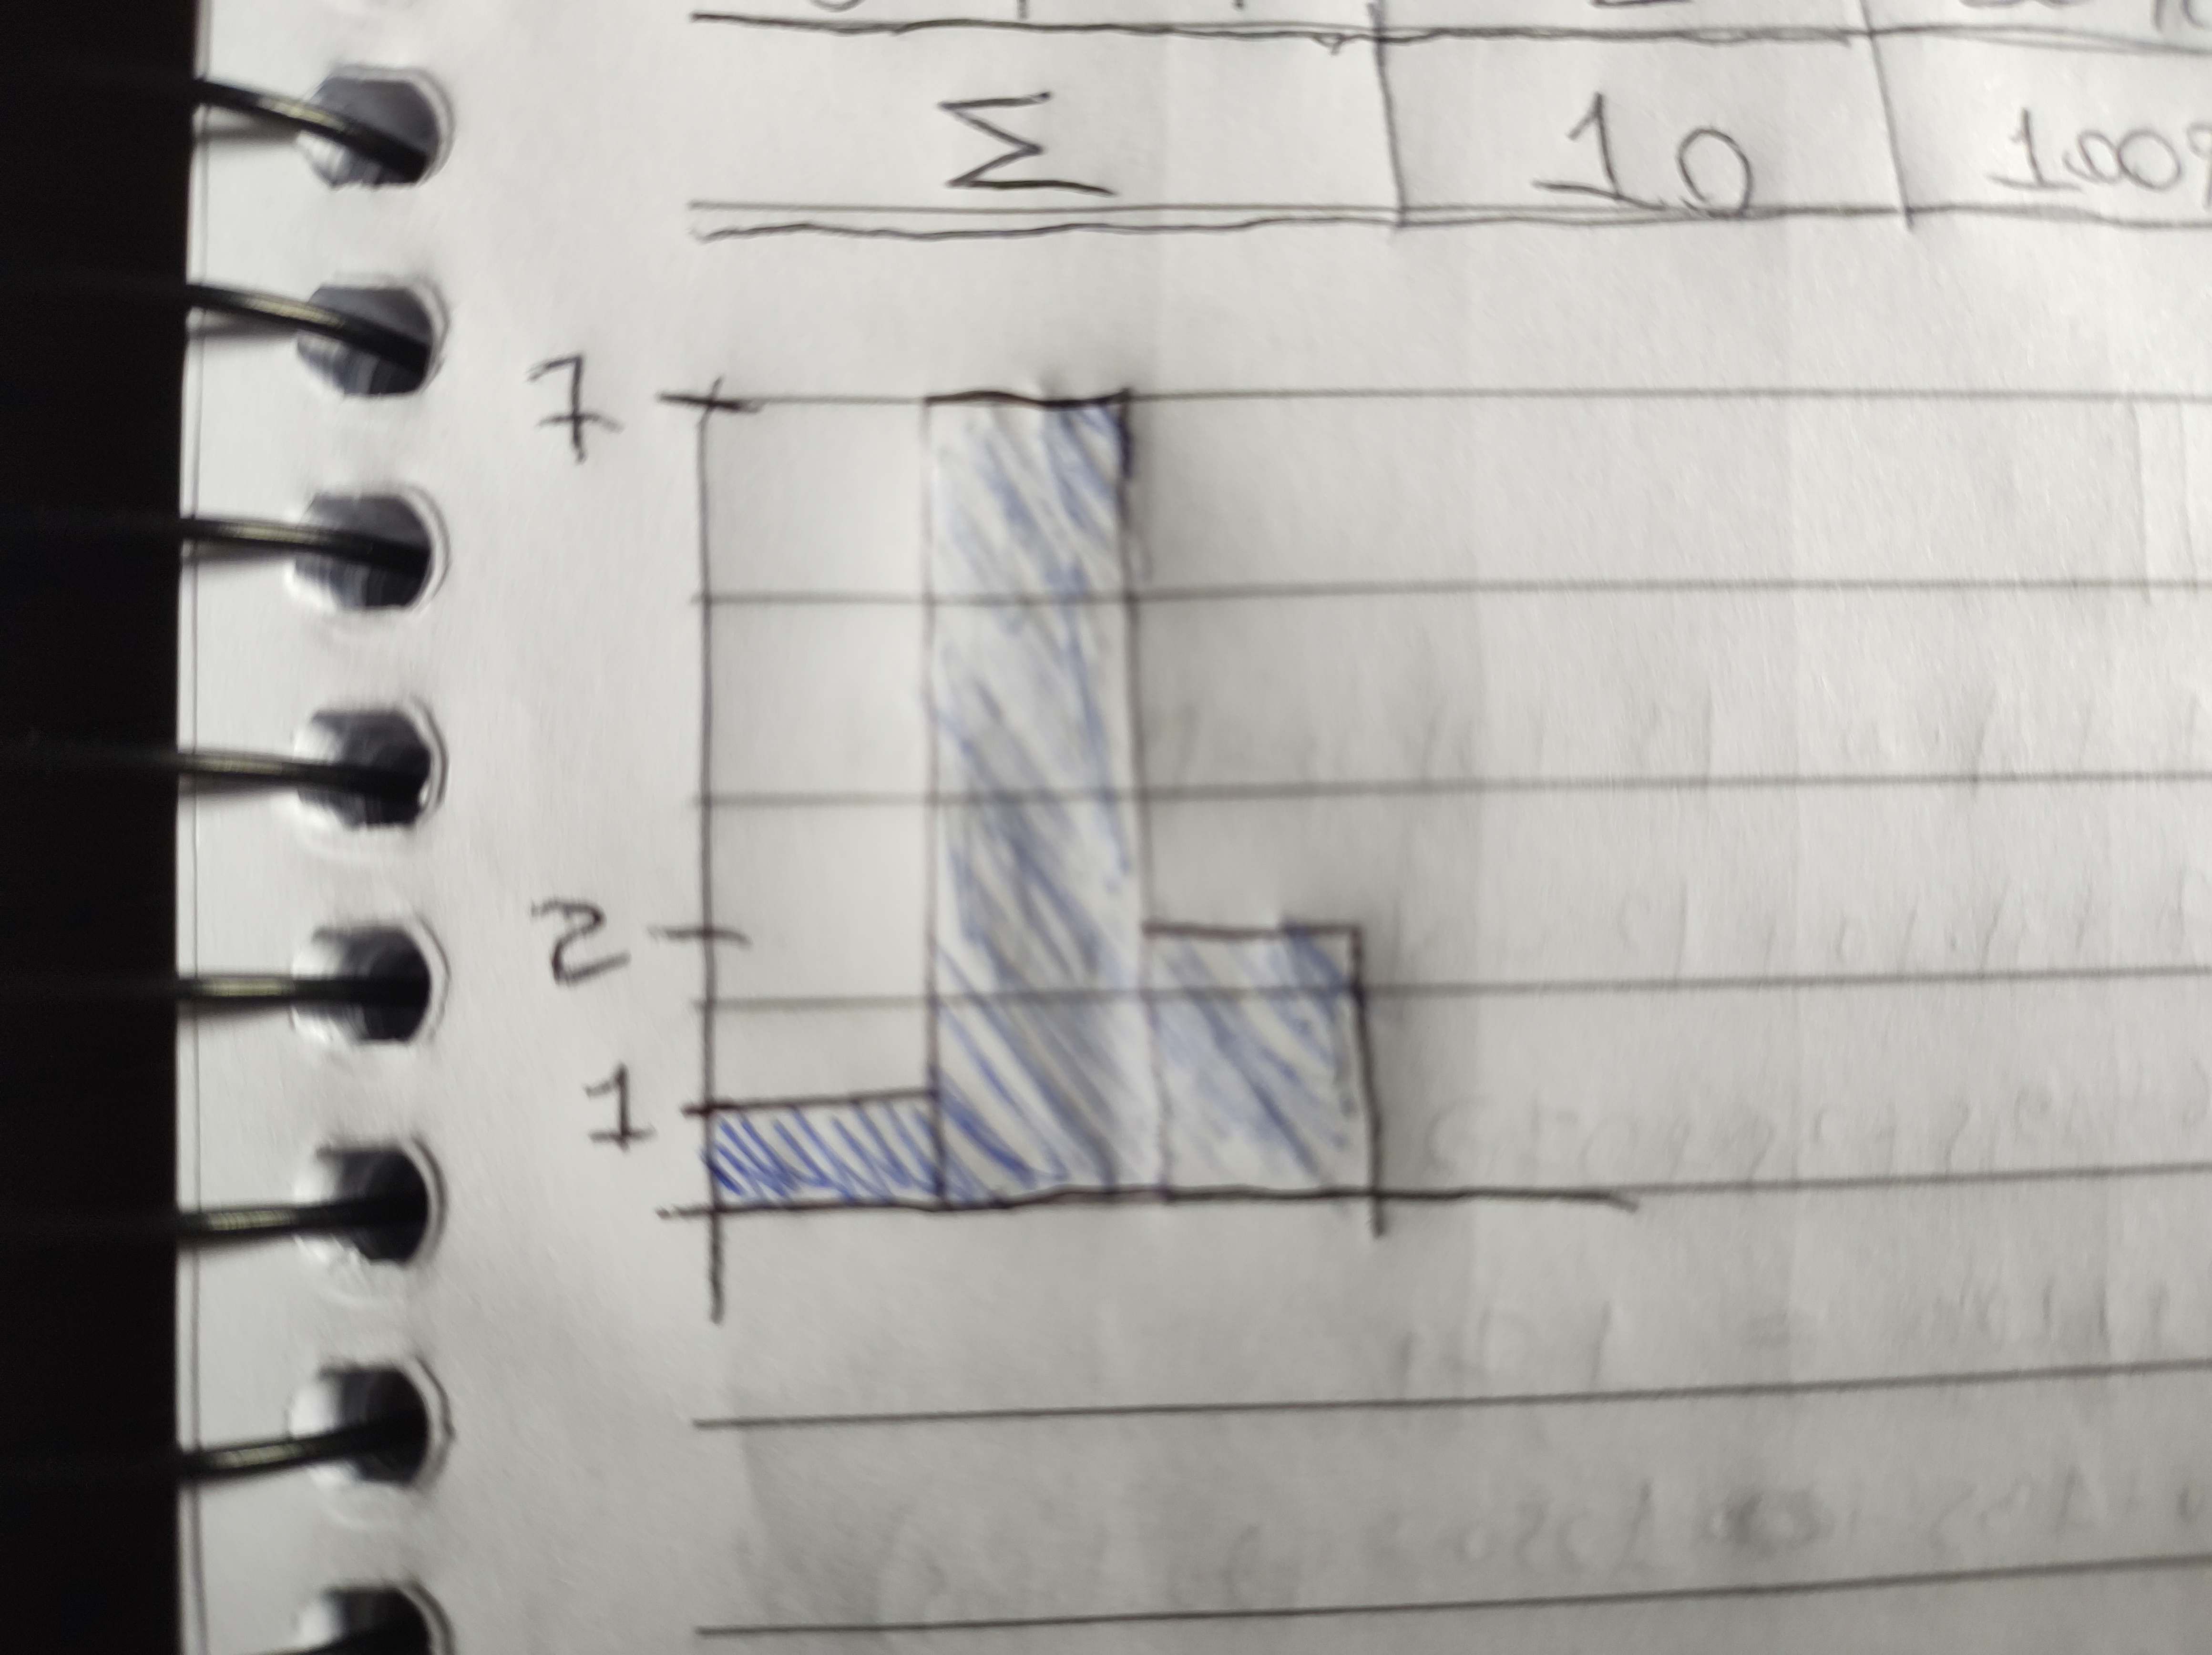
\includegraphics[scale=0.05]{q2d}
	\end{figure}
\par (e) observa-se que ocorre pouca variação dos dados, exceto pelos valores outliers 1.4, 3.7 e 3.9, que amentam os desvios.
\vspace{+6pt}
\par $DM = \dfrac{\sum_{1}^{10}|X_i-\overline{X}|}{n} = 0.528$
\vspace{+6pt}
\par $S^2 = \dfrac{\sum_{1}^{10}{X_i-\overline{X}}^2}{n-1} = 0.5832$
\vspace{+6pt}
\par $S = \sqrt{0.5832} = 0.7636$
\vspace{+6pt}
\par $CV = \dfrac{S}{\overline{X}} = 0.3066$
\vspace{+6pt}
\par (f) a média é um representativo do todo, nos permite saber um bom valor aleatório caso fosse adicionado outro valor a tabela, porém ela leva em considerações os extremos como 3.9, 3.7 e 1.4, sendo um pouco mais alta do esperado sem estes outliers, pode ser avaliada usando as medidas de dispersão acima
\par (g) usar os índices de variância, desvio padrão e coeficiente de variação porém com a média harmônica e geométrica nas equações ao invés da média aritmética.
\par (h) o coeficiente de assimetria positivo nos permite saber que a maior parte dos dados está concentrado a esquerda, a curtose positiva dá a informação que o gráfico é mais centralizado em uma parte.
\vspace{+6pt}
\par $A_s = (\sqrt{\dfrac{n}{n-1}})(\dfrac{1}{n-1})\dfrac{\sum_{1}^{10}{X_i-\overline{X}}^3}{S^3} = 0.7924$
\vspace{+6pt}
\par $ K = (\dfrac{n}{{n-1}^2})(\dfrac{\sum_{1}^{10}{x_i-\overline{X}}^4}{S^4}) - 3 = 0.942154$
\vspace{+12pt}
\par \textbf{Questão 3}
\vspace{+12pt}
\par (a)
	\begin{figure}[h!]
		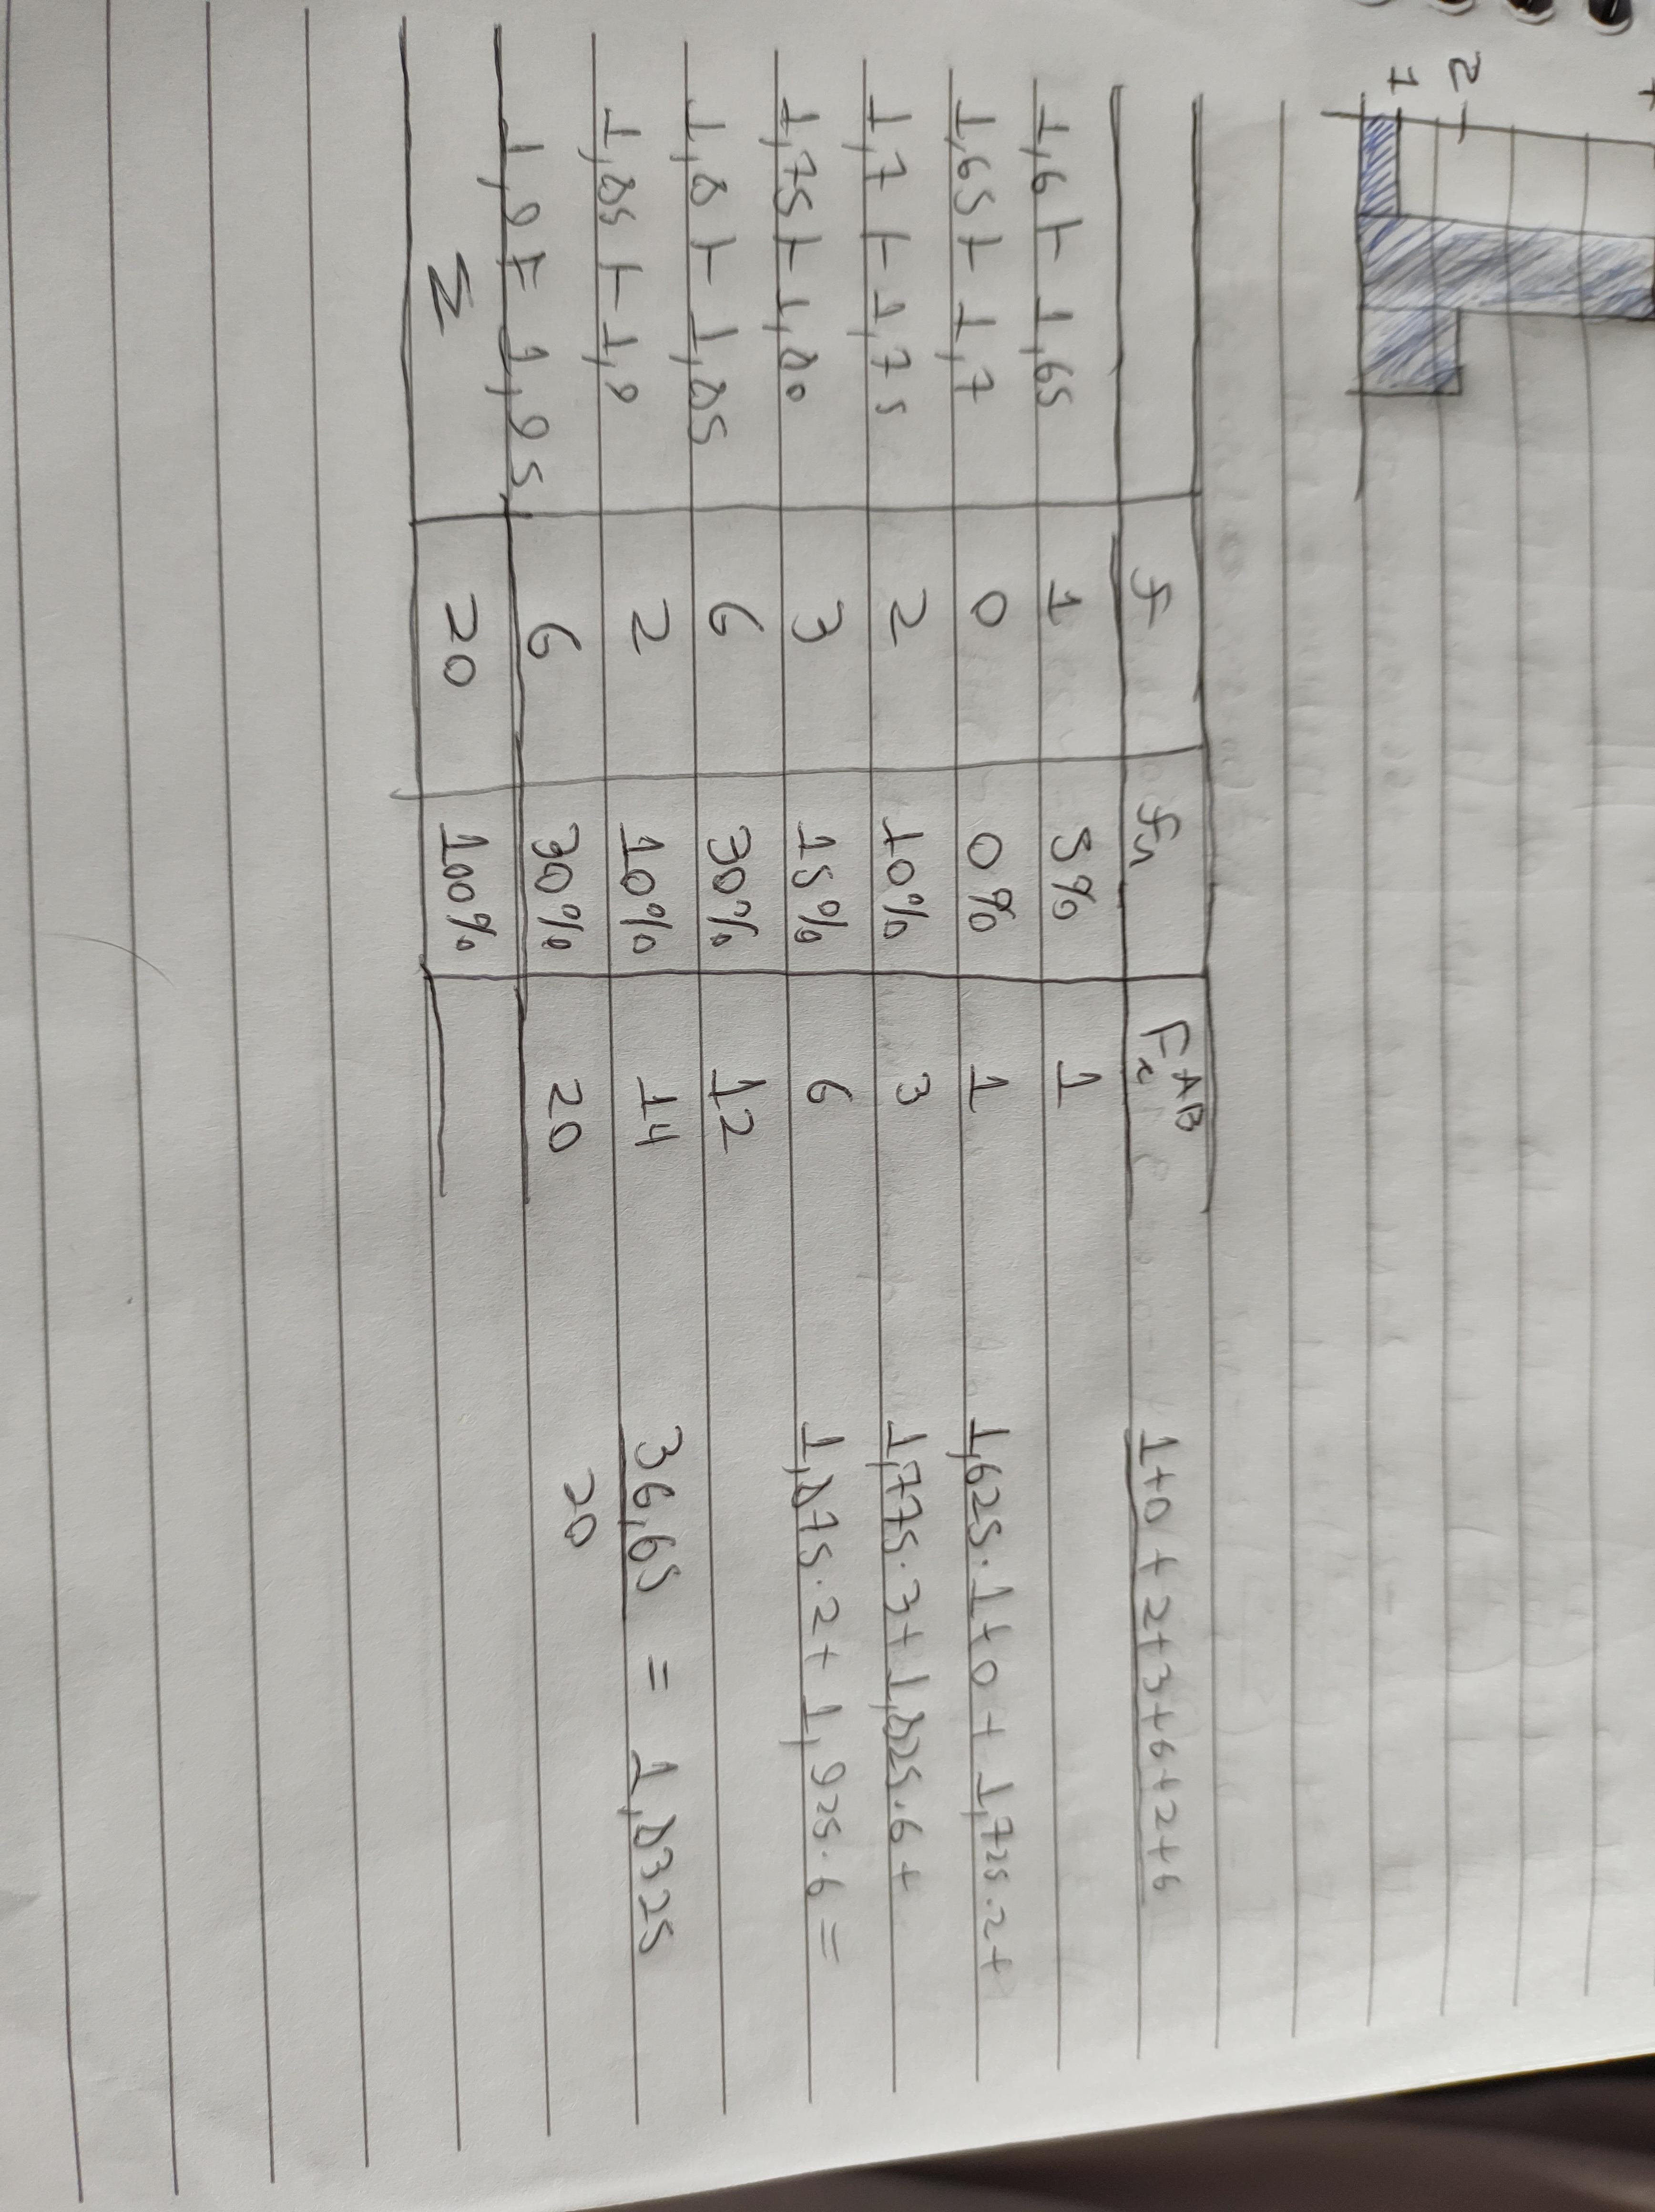
\includegraphics[scale=0.07]{q3a}
	\end{figure}
\par (b) $14/20 = 70\%$ dos atletas
\par (c) sim, é possível perceber que os dados estão mais concentrados a esquerda, entre os valores 1.65 e 1.88, com uma diferença entre os quartis e máximos e mínimos maiores na parte direita do gráfico.
	\begin{figure}[h!]
		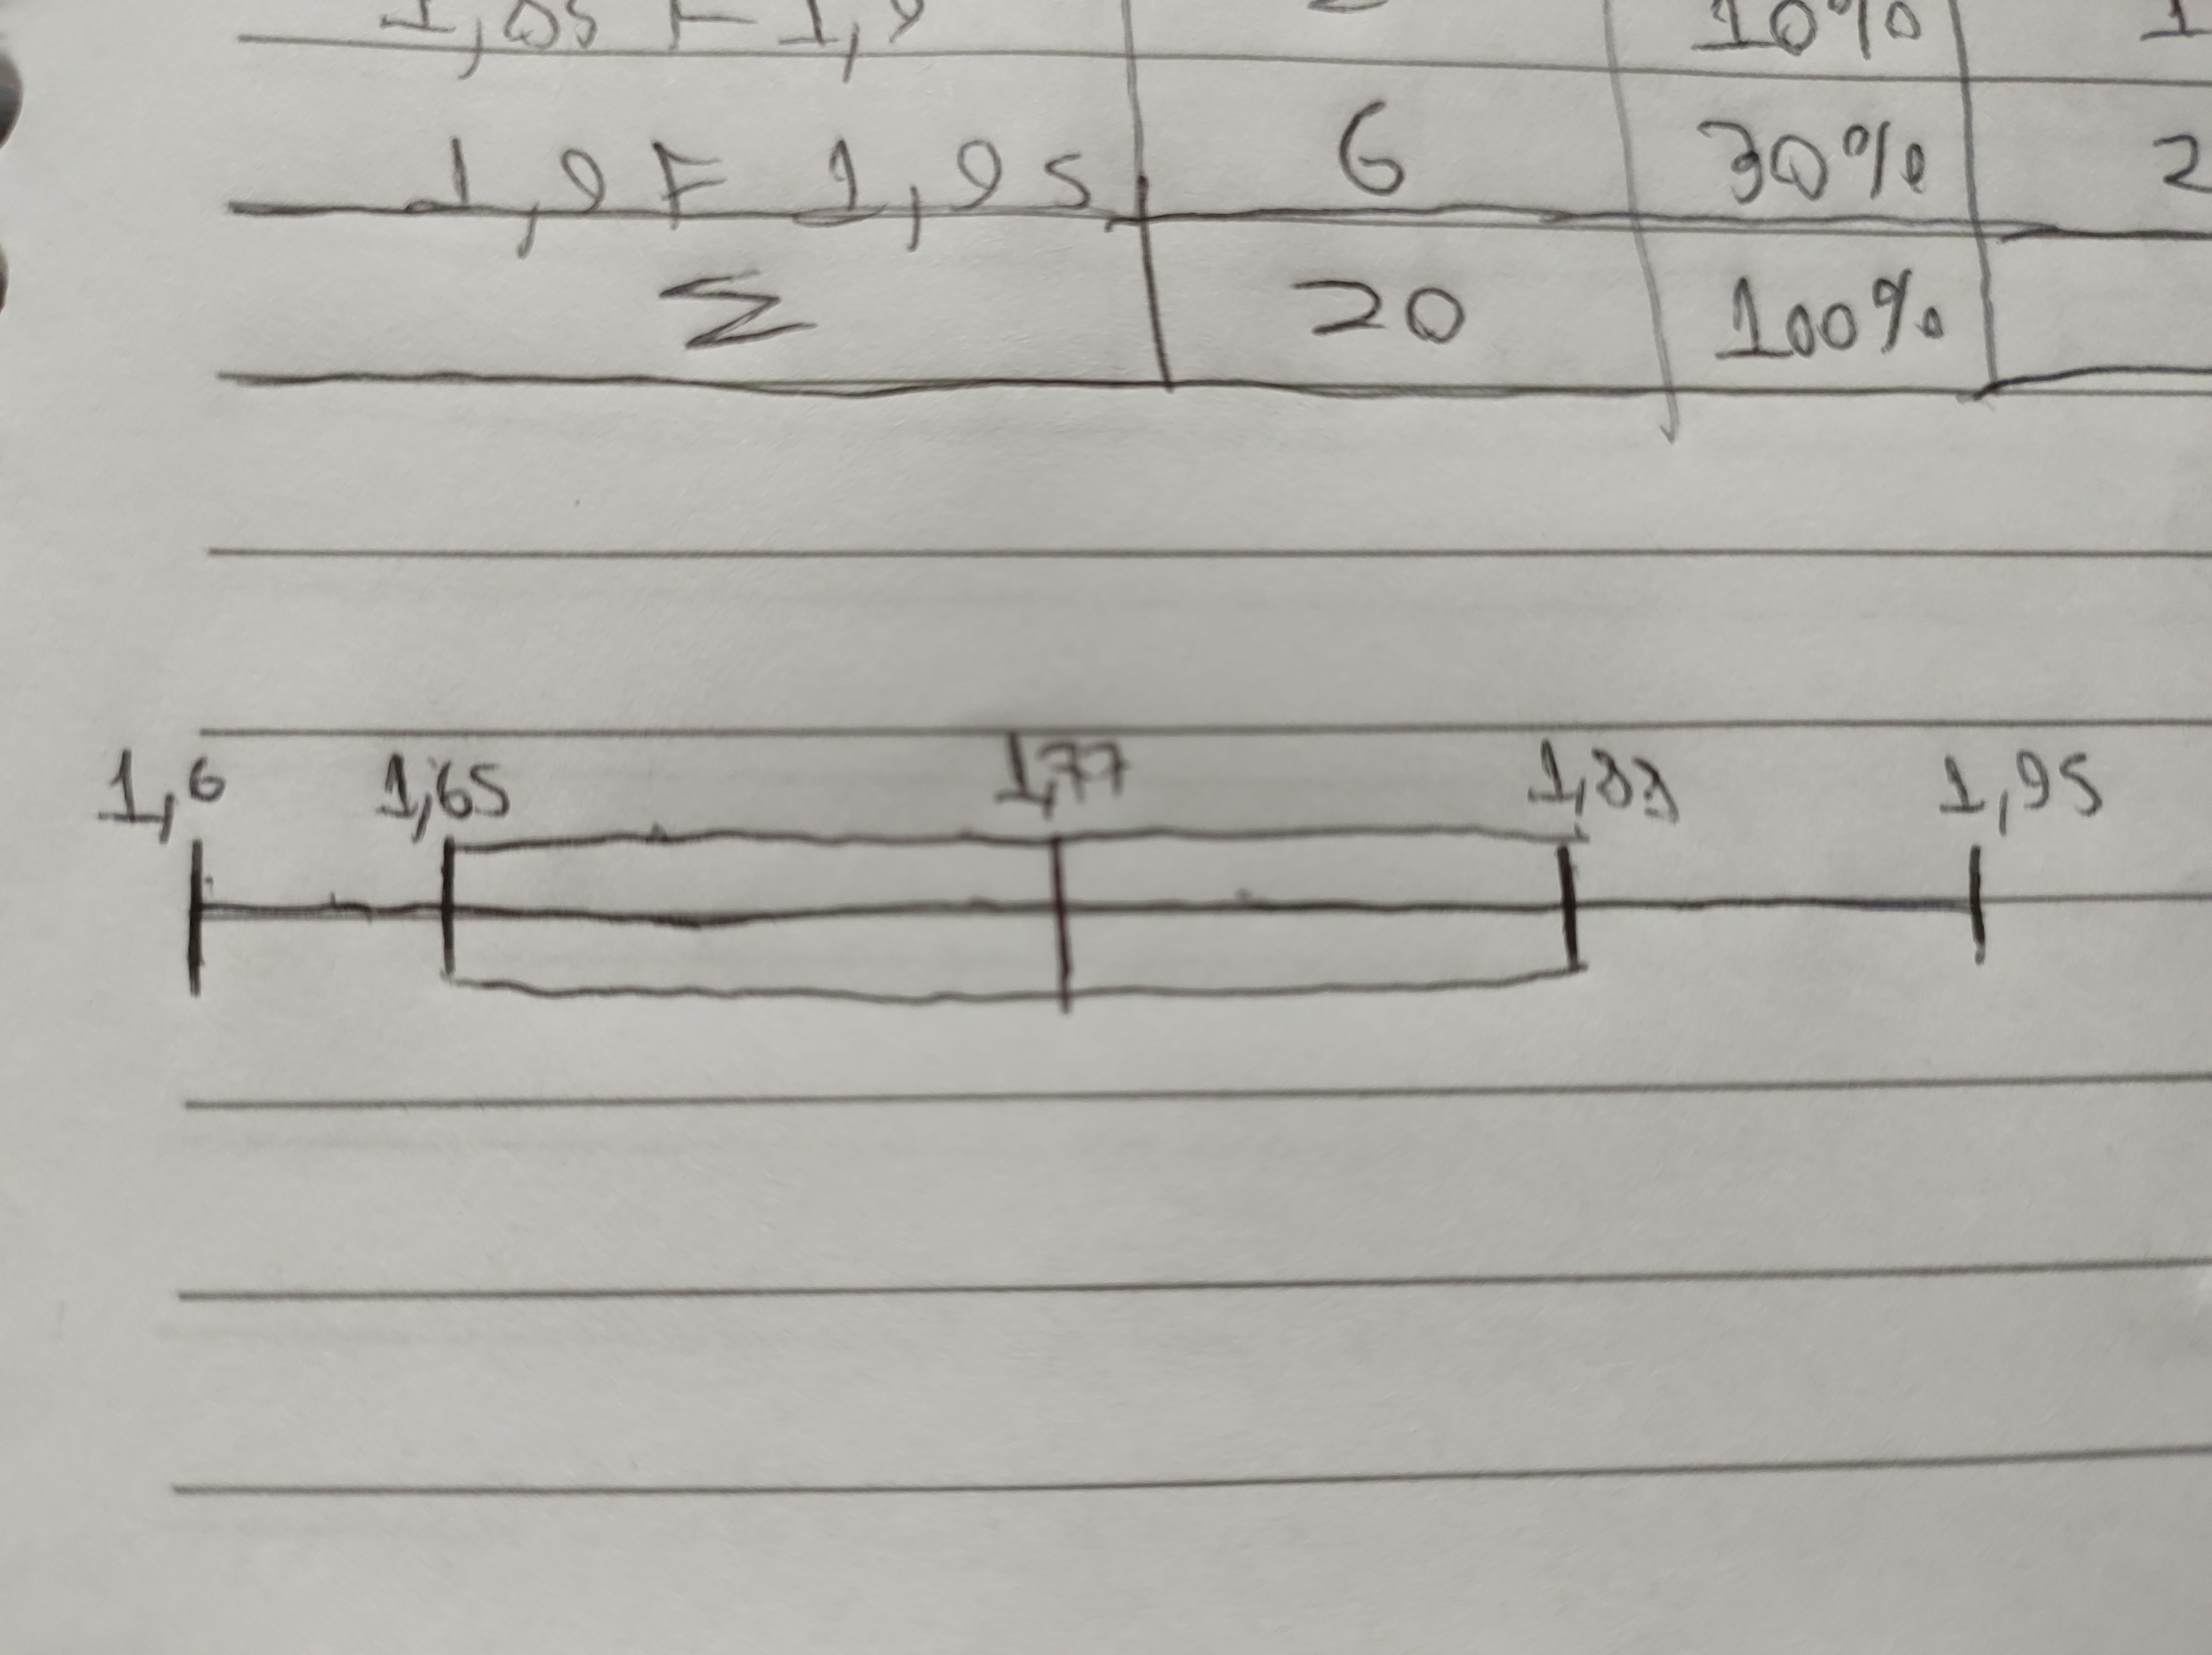
\includegraphics[scale=0.03]{q3c}
	\end{figure}
\vspace{+12pt}
\par \textbf{Questão 4}
\vspace{+12pt}
\par sim, todas as afirmações estão certas, já que $a$ é uma constante não referenciada no somatório em $n$, podendo ser movida para fora dos somatórios.
\vspace{+6pt}
\par $a*\overline{X_a} = \dfrac{\sum_{1}^{n}a*x_i}{n}$
\vspace{+6pt}
\par $\Rightarrow a*\overline{X_a} = \dfrac{a*\sum_{1}^{n}x_i}{n}$
\vspace{+6pt}
\par $\Rightarrow a*\overline{X_a} = a *  \dfrac{\sum_{1}^{n}x_i}{n}$
\vspace{+6pt}
\par $\Rightarrow \overline{X_a} = \dfrac{\sum_{1}^{n}x_i}{n}$ Q.E.D.
\vspace{+6pt}
\par o mesmo pode ser feito para média geométrica, harmônica e quadrática
\vspace{+12pt}
\par \textbf{Questão 5}
\vspace{+12pt}
\par letra (b) esta correta, pois a posição da mediana nesta tabela $n=100$ será $X_{(\frac{50+51}{2})}$, que através das frequências pode se notar que estará presente no intervalo de classes $10 \vdash 20$, alternativamente:
\vspace{+6pt}
\par $M_d = LI_{md} + (\dfrac{E_{md}-F_{ant}^{ab}}{f_{md}})*h$
\vspace{+6pt}
\par $M_d = 10 + (\dfrac{50-47}{29})*10$
\vspace{+6pt}
\par $M_d = 10 + 30/29$
\vspace{+6pt}
\par $M_d = 11.03$, contido na classe $10 \vdash 20$
\end{document}